\section{Метод компенсации нелинейных искажений на приемнике}
Компенсация нелинейных искажений сигнала является важным этапом для
сохранения производительности системы. С расширением стандарта связи 5G NR
в миллиметровый диапазон, компенсация становится особенно актуальной,
поскольку характеристики усилителей в этом диапазоне значительно хуже, чем
для более низких частот.

\subsection{Обзор существующих решений}
На текущий момент были исследованы несколько основных подходов для
компенсации нелинейных искажений, они разделяются на два основных
направления.

\subsubsection{Обработка сигнала на передатчике}

Первый заключается в предварительном искажении сигнала перед
подачей на УМ на передатчике. Сигналу придаются свойства, которые
минимизируют влияние нелинейного искажения от УМ, эффективно "выпрямляя"
его АХ. Существует множество вариантов обработки для данного подхода,
однако многие из них имеют слабый эффект на общей производительности
системы, а подход с применением предварительного искажения сигнала имеет
низкую эффективность при низких значениях IBO, при которой достигается
максимальная эффективность усилителя \cite{sharath2015}
\cite{shabany2008} \cite{eda2001}. Также, использование PD на передатчике
нежелательно на мало-габаритных устройствах, поскольку в таком случае
увеличивается сложность устройства, объем сигнальной обработки и энергопотребление.

\subsubsection{Обработка сигнала на приемнике}

Второй основной подход заключается в компенсации нелинейных искажений на
приемнике. Например, в работе \cite{maltsev2021} используется
статистическая обработка принятого сигнала для определения степени
искажения, на основе которой в дальнейшем производится компенсация. Многие
работы \cite[]{sharath2015, shabany2008,bhat2016,qi2010,gregorio2007,
bouhadda2015,drotar2010} рассматривают теоретический подход для компенсации
на приемнике в очень обобщенном случае. Несколько методов компенсации были
предложены для OFDM сигнала \cite[]{gregorio2007,bouhadda2015, drotar2010},
где влияние нелинейности представляется комплексным множителем, а также
Гауссовой шумовой компонентой. Основной задачей в таком случае является
определение параметров УМ (они могут быть как известны изначально, так и
определены с помощью пилотных сигналов) для компенсации нелинейного
искажения. Несколько методов были исследованы для сигнала SC с одной несущей
(\textit{Англ. - SC - Single Carrier}) \cite[]{sharath2015,
shabany2008,bhat2016, qi2010}, в частности использовалась обратная
характеристика УМ и последовательные методы Монте-Карло. В нескольких
случаях \cite[]{bhat2016, qi2010,gregorio2007}, значения параметров УМ
считаются известными на приемнике, что позволяет произвести компенсацию
искажения. В случаях, когда параметры УМ оцениваются, производительность
такая же либо хуже.

В данной работе описывается метод компенсации нелинейных искажений УМ на
приемнике с использованием обратной амплитудной характеристики. Информация
о параметрах и рабочей точке усилителя предполагается известной. Работа и
эффективность метода будет исследоваться на существующем симуляторе
канального уровня, необходимые изменения будут вноситься в код симулятора
как для внесения искажений, так и для их компенсации.



\subsection{Краткое описание архитектуры LLS системы мобильной связи}

Для исследования влияния нелинейности УМ в диапазонах частот 30-70 ГГц и
100-200 ГГц, а также проверки работоспособности разработанного метода
компенсации нелинейных искажений на приемнике, в работе использовался
полноценный симулятор канального уровня LLS (\textit{Англ. - Link Level
Simulator}), соответствующий требованиям стандарта 5G NR 3GPP. В этой части
работы будут кратко описаны принципы работы, архитектура и основные
составляющие LLS. 

На рис. \ref{fig:lls_scheme} приведена принципиальная схемы работы LLS.
\begin{figure}[h!]
    \centering
    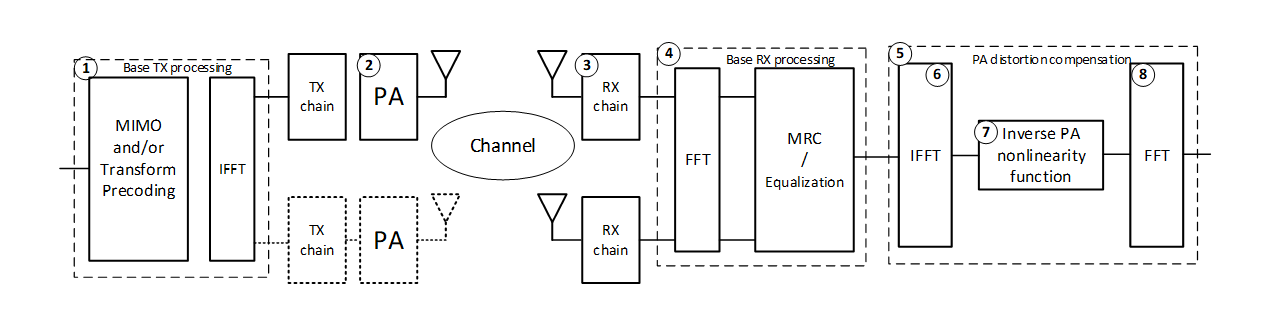
\includegraphics[width=0.99\linewidth]{figs/lls_scheme.png}
    \caption{}
    \label{fig:lls_scheme}
\end{figure}

TBD

% Схема компенсации состоит из базовой обработки на передатчике (1),
% которая может включать MIMO прекодинг и transform прекодинг (в случае
% DFT-s-OFDM сигнала),  а также стандартного для OFDM блока обратного
% преобразования Фурье. Сгенерированный OFDM сигнал подается на одну или
% более передающих цепочек, которые могут включать добавление цикличного
% префикса, перенос сигнала на несущую частоту, и, наконец, сигнал подается
% на усилитель мощности (2), работающий на несущей частоте. Отметим, что
% для корректной работы предлагаемой схемы, сигналы на разных антеннах
% должны иметь одинаковую амплитуду (но могут иметь разную фазу). Это
% ограничивает применение данного метода до передачи 1 ранга, даже если
% используется несколько передающих антенн. После прохождения через канал,
% сигнал попадает на приемную цепь состоящую из одной или нескольких
% приемных антенн для дальнейшей обработки (4), которая может состоять из
% преобразования Фурье further maximum ration combining (MRC) and frequency
% domain equalization???. Такая обработка эффективно нивелирует влияние
% частотно-селективного канала, что позволяет использовать обработанный
% сигнал на блоке компенсации нелинейного искажения (5). Этот блок может
% состоять из операции обратного Фурье преобразования (6) для возвращения
% сигнала во временную область, блока обратной нелинейной функции УМ (7),
% который выполняет компенсацию нелинейного искажения, а также блока
% прямого преобразования Фурье для возвращения сигнала в частотную область.






\subsection{Влияние нелинейных искажений в LLS на качество приема}

\begin{figure}[h!]
    \centering
    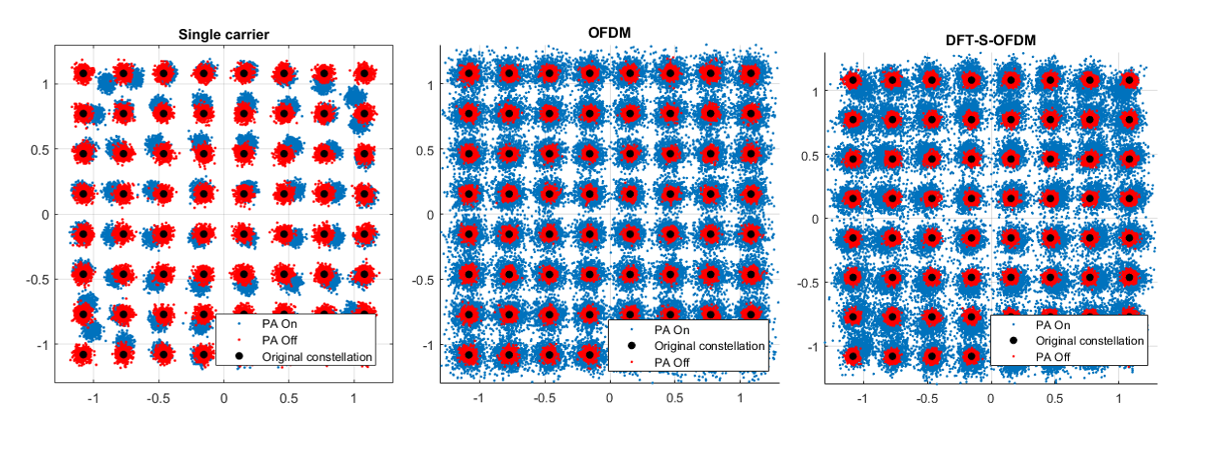
\includegraphics[width=0.95\linewidth]{figs/ofdm_pa_distortions.png}
    \caption{Искажение различных сигналов на приемнике при внесении нелинейного
    искажения на передатчике}
    \label{fig:lls_rapp_distortions}
\end{figure}

\subsection{Подход и описание нового метода компенсации нелинейных искажений}
В основе разработанного метода компенсации нелинейных искажений на
приемнике лежит использование обратной АХ усилителя. Параметры $G, V_{sat},
p$, необходимые для восстановления обратной характеристики считаются
известными. Помимо этих параметров, важно также знать рабочую точку УМ,
поскольку это напрямую влияет на степень искажения принятого сигнала.
Рабочая точка также считается известной. Компенсация будет производиться
в основном для амплитудных искажений, поскольку фазовые искажения незначительны.

Принципиальный подход компенсации искажений может быть описан следующим
образом:
\begin{enumerate}
    \item Принятый сигнал проходит через предварительную обработку в LLS
    (частотное выравнивание, MIMO-декодирование, перенос в частотную
    область)
    \item Полученный обработанный сигнал в частотной области переносится во
    временную область в соответствии с используемым типом сигнала.
    \subitem Transform precoding (в случае DFT-s-OFDM сигнала)
    \subitem IFFT-обработка для получения OFDM сигнала во временной области
    \item Полученный сигнал во временной области подается на блок
    компенсации (использующий обратную АХ усилителя на основе известных
    параметров и рабочей точки)
    \item Сигнал с компенсированными искажениями переводится в частотную
    область
    \item Компенсированный сигнал подается на блок демодуляции
\end{enumerate}

Блок-схема разработанного метода компенсации приведена на рис.
\ref{fig:compensation_scheme}. 

\begin{figure}[h!]
    \centering
    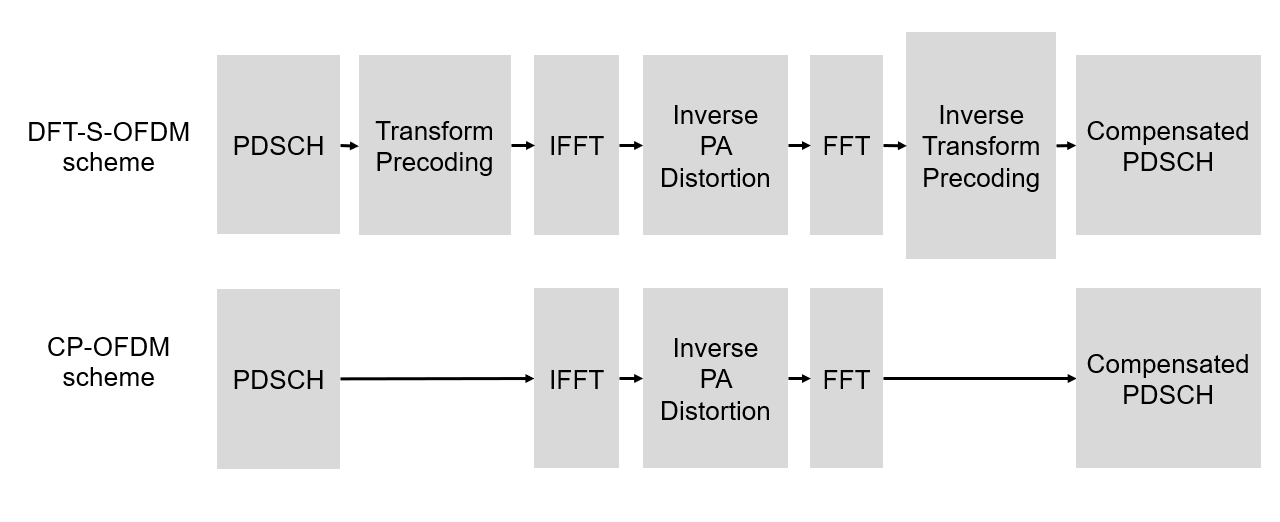
\includegraphics[width=0.95\linewidth]{figs/compensation_scheme.png}
    \caption{}
    \label{fig:compensation_scheme}
\end{figure}


\subsubsection{Компенсация с использованием обратной характеристики усилителя}

Для компенсации нелинейных искажений важно понимать как именно искажается
сигнал на передатчике. Перед подачей на УМ сигнал, сформированный в
частотной области, преобразуется в OFDM сигнал во временной области
посредством IFFT. После этого OFDM сигнал подается на УМ и далее на
передающие антенны. Таким образом, искажение сигнала происходит во
временной области, следовательно, компенсация также должна производиться во
временной области. 

Поскольку в LLS сигнал после передачи проходит через частотно-селективный
канал, одним из первых шагов является частотное выравнивание с
помощью опорных сигналов DMRS, помещенных в передаваемый сигнал на этапе
подготовки перед передачей. Эти сигналы доступны в частотной области,
поэтому принятый OFDM сигнал проходит через блок FFT. Происходит перенос в
частотную область, где выполняется частотное выравнивание сигнала.

Дальнейший перенос искаженного сигнала во временную область для выполнения
компенсации происходит посредством выполнения обработки, идентичной
обработке сигнала на передатчике. Например, для CP-OFDM сигнала необходимо
провести преобразование IFFT. В таком случае преобразованный сигнал
становится приближенным к сигналу на выходе УМ, и появляется возможность
применить обратную АХ усилителя для компенсации. Обратная характеристика УМ
может быть получена из модели Раппа \ref{eq:Rapp}. Результирующее выражение
приведено в \ref{eq:invRapp}.


\begin{equation}
    \displaystyle
    F^{-1}_{AM/AM}(y) = 
       \frac{ y}{\left( 1 - \abs{\frac{y}{V_{sat}}}^{2p}\right)^{1/2p}},
    \label{eq:invRapp}
\end{equation}
где $y$ - сигнал на приемнике после переноса во временную область. 


В ходе исследований изначально использовалась обратная АХ УМ, приведенная в
\ref{eq:invRapp}. Усилитель по своей природе имеет свойство выходить на
насыщение после определенного уровня подаваемой мощности, т.е. после
определенного момента, в независимости от увеличения подаваемой мощности,
выходная мощность не будет расти. Это отражается в АХ в виде выхода на
уровень насыщения, связанного с параметром $V_{sat}$. При этом обратная
характеристика $F^{-1}_{AM/AM}$ стремится к бесконечности при приближении
входного значения к $V_{sat}$, т.е.:
\begin{equation}
    F^{-1}_{AM/AM}(y) \rightarrow \infty \eval_{y \rightarrow V_{sat}}
\end{equation}
Подобное поведение может привести к дополнительным искажениям
компенсируемого сигнала, что противоречит изначальной цели. OFDM сигнал
имеет высокое значение PAPR, поэтому при подаче на обратную характеристику
УМ \ref{eq:invRapp}, некоторые значения могут быть больше $V_{sat}$, что
невозможно физически. Этот эффект может привести к дополнительным
искажениям, пример таких искажений приведен на центральном графике рис.
\ref{fig:inf_distortion}.

\begin{figure}[h!]
    \centering
    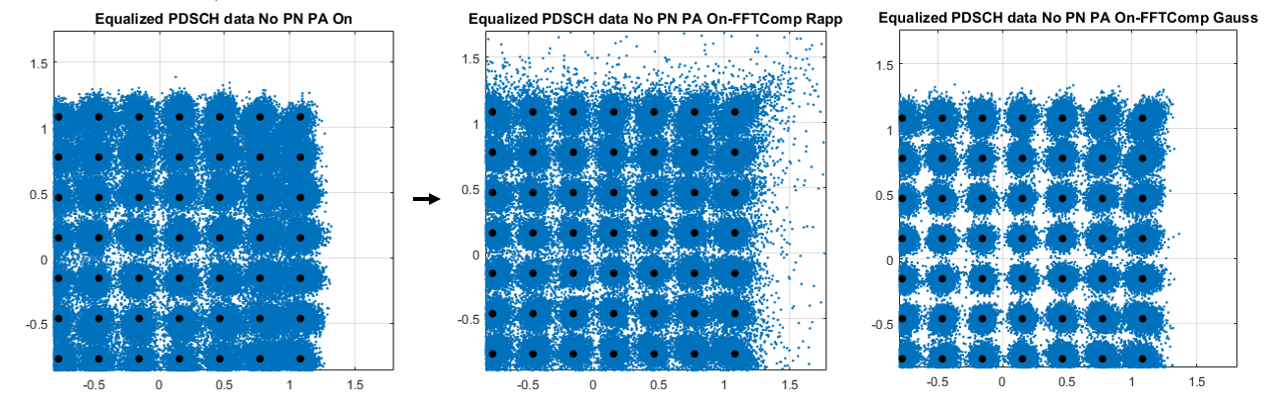
\includegraphics[width=0.9\linewidth]{figs/ceiled_rapp_result.png}
    \caption{Результат применения обратной АХ \ref{eq:invRapp} и
    ограниченной обратной АХ \ref{eq:invCeiledRapp} к DFT-s-OFDM сигналу
    для компенсации. Черные точки отображают точки изначальное,
    передаваемое созвездие, синие точки обозначают значения созвездия
    принятого сигнала на приемнике. На графике слева компенсация
    отсутствует, по центру компенсация выполнена не ограниченной обратной
    АХ \ref{eq:invRapp}, справа ограничено обратной АХ
    \ref{eq:invCeiledRapp}. Поскольку на центральном графике обратная
    функция не ограничена, результирующее созвездие имеет дополнительно
    искажение в областях значений с высокой амплитудой. При ограничении
    обратной характеристики наблюдается необходимая компенсация искажений.}
    \label{fig:inf_distortion}
\end{figure}

Таким образом важно произвести модификацию обратной характеристики,
ограничив ее значения при $y \rightarrow V_{sat}$. В результате было
получено выражение, приведенное в \ref{eq:invCeiledRapp}. Сравнение
результата применения ограниченной и не ограниченной характеристик
приведено на рис. \ref{fig:inf_distortion}. В дальнейшем в работе
использовалась именно ограниченная версия обратной АХ \ref{eq:invCeiledRapp}.

\begin{equation}
    F^{-1}_{AM/AM}(y) = 
    \begin{cases}
        \displaystyle
       \frac{ y}{\left( 1 - \abs{\frac{y}{V_{sat}}}^{2p}\right)^{1/2p}}
       \quad y <\alpha V_{sat}\\
       \frac{ \alpha V_{sat}}{\left( 1 - \abs{\alpha}^{2p}\right)^{1/2p}}
       \quad y \geq \alpha V_{sat}
    \end{cases},
    \label{eq:invCeiledRapp}
\end{equation}




TBD





\subsubsection{Адаптация алгоритма компенсации в зависимости от типа используемого сигнала}
Возможность обработки нескольких типов сигнала.